\newif\ifpublic
\publictrue

\documentclass[conference]{IEEEtran}

% Make sure that we have page numbers
\thispagestyle{plain}
\pagestyle{plain}

\IEEEoverridecommandlockouts % this enables the \thanks command

\usepackage{epsfig}
\usepackage{setup}


% \newtheorem{theorem}{Theorem}[section]
% \newtheorem{lemma}[theorem]{Lemma}
% \newtheorem{corollary}[theorem]{Corollary}
% \newtheorem{dfn}[theorem]{Definition}
% \newtheorem{hypothesis}[theorem]{Hypothesis}

\newcommand\invisiblesection[1]{%
  \refstepcounter{section}
\sectionmark{#1}}

% \newenvironment{proof}[1][Proof]{\begin{trivlist}
% \item[\hskip \labelsep {\bfseries #1}]}{\end{trivlist}}
%   \newenvironment{definition}[1][Definition]{\begin{trivlist}
% \item[\hskip \labelsep {\bfseries #1}]}{\end{trivlist}}
%   \newenvironment{example}[1][Example]{\begin{trivlist}
% \item[\hskip \labelsep {\bfseries #1}]}{\end{trivlist}}
%   \newenvironment{remark}[1][Remark]{\begin{trivlist}
% \item[\hskip \labelsep {\bfseries #1}]}{\end{trivlist}}

% \newcommand{\qed}{\nobreak \ifvmode \relax \else
%   \ifdim\lastskip<1.5em \hskip-\lastskip
%   \hskip1.5em plus0em minus0.5em \fi \nobreak
% \vrule height0.75em width0.5em depth0.25em\fi}

\newcommand{\sref}[1]{Section~\ref{#1}}
\newcommand{\tref}[1]{Theorem~\ref{#1}}
\newcommand{\lref}[1]{Lemma~\ref{#1}}
\newcommand{\fref}[1]{Figure~\ref{#1}}
\newcommand{\aref}[1]{Algorithm~\ref{#1}}
\newcommand{\N}{\ensuremath{\mathbb{N}}\xspace}
\newcommand{\Z}{\ensuremath{\mathbb{Z}}\xspace}
\newcommand{\K}{\ensuremath{\mathbb{K}}\xspace}
\renewcommand{\L}{\ensuremath{\mathbb{L}}\xspace}
\newcommand{\corr}{\,\hat{=}\,}
\newcommand{\Oinf}{\ensuremath{\mathcal{O}}\xspace}
\newcommand{\F}[1]{\ensuremath{\mathbb{F}_{#1}}\xspace}
\newcommand{\mbf}{\ensuremath{\mathbf}}
\newcommand{\ie}{{\textit{i.e.}},\;}
\newcommand{\eg}{{\textit{e.g.}},\;}
\newcommand{\p}{\ensuremath{2^{255}-19}}
\newcommand{\Zfield}{\ensuremath{\mathbb{Z}_{\p}}}
\newcommand{\Ffield}{\ensuremath{\mathbb{F}_{\p}}}
\newcommand{\xcoord}{$x$-coordinate\xspace}
\newcommand{\xcoords}{$x$-coordinates\xspace}


\begin{document}


\title{\Large \bf A Coq proof of the correctness of X25519 in TweetNaCl}
\date{}

\ifpublic
    \author{
        \IEEEauthorblockN{Peter Schwabe}
        \IEEEauthorblockA{MPI-SP, Germany \&\\
        Radboud University, The Netherlands}
        \and
        \IEEEauthorblockN{Beno\^it Viguier}
        \IEEEauthorblockA{Radboud University,\\
        The Netherlands}
        \and
        \IEEEauthorblockN{Timmy Weerwag}
        \IEEEauthorblockA{Radboud University,\\
        The Netherlands}
        \and
        \IEEEauthorblockN{Freek Wiedijk}
        \IEEEauthorblockA{Radboud University,\\
        The Netherlands}
    }
\else
    \author{}
\fi

\maketitle

% \subsection*{Abstract}
\begin{abstract}

  In this paper we formally prove that the C implementation of
  X25519 key exchange in the TweetNaCl library matches
  the mathematical definition of X25519 from Bernstein's 2006 paper.
  The proof is computer-verified using the Coq theorem prover.
  To establish the link between C and Coq we use the 
  Verified Software Toolchain (VST).

\end{abstract}


NaCl~\cite{BLS12} is an easy-to-use high-security high-speed software library
for network communication, encryption, decryption, signatures, etc.
TweetNaCl~\cite{BGJ+15} is its compact reimplementation.
It does not aim for high speed application and has been optimized for source
code compactness (100 tweets). It maintains some degree of readability in order
to be easily auditable.
TweetNaCl is being used by ZeroMQ~\cite{zmq} messaging queue system to provide
portability to its users.
``TweetNaCl is the
first cryptographic library that allows correct functionality to be verified
by auditors with reasonable effort''~\cite{BGJ+15}

% XXX: TweetNaCl (find real-world use of TweetNaCl?)
% Mega.nz uses tweetnacl-js (as JS port of tweetnacl) for their webclient https://mega.nz/
% Keybase client: https://github.com/keybase/node-nacl/blob/master/lib/tweetnacl.js

One core component of TweetNaCl (and NaCl) is the key exchange protocol X25519~\cite{rfc7748}.
This protocol is being used by a wide variety of applications~\cite{this-that-use-curve25519}
such as SSH~\cite{rfc4253}, Signal Protocol, Tor, Zcash, TLS to establish a shared secret over
an insecure channel.

This library makes use of Curve25519~\cite{Ber06}, a function over a \F{p}-restricted
$x$-coordinate computing a scalar multiplication on $E(\F{p^2})$, where $p$ is
the prime number $\p$ and $E$ is the elliptic curve $y^2 = x^3 + 486662 x^2 + x$.

Originally, the name ``Curve25519'' referred to this keyexchange protocol,
but Bernstein suggested to rename the scheme to X25519 and to use the name
Curve25519 for the underlying elliptic curve~\cite{Ber14}.
We make use of this notation in this paper.

\subheading{Contribution of this paper}


\todo{Proof that TweetNaCl's X25519 code correctly implements math definition from 25519 paper}

\todo{State additional contributions, e.g., extension of EC framework by Bartiza and Strub.}

Implementing cryptographic primitives without any bugs is difficult.
While tests provides with code coverage, they still don't cover 100\% of the
possible input values. In order to get formal guaranties a software meets its
specifications, two methodologies exist.

The first one is by synthesizing a formal specification and generating machine
code by refinment in order to get a software correct by construction.
This approach is being used in e.g. the B-method~\cite{Abrial:1996:BAP:236705},
F*~\cite{DBLP:journals/corr/BhargavanDFHPRR17}, or with Coq~\cite{CpdtJFR}.

However this first method cannot be applied to an existing piece of software.
In such case we need to write the specifications and then verify the correctness
of the implementation.

\subheading{Our Formal Approach.}
Verifying an existing cryptographic library, we use the second approach.
Our method can be seen as a static analysis over the input values coupled
with the formal proof that the code of the algorithm matches its specification.

We use Coq~\cite{coq-faq}, a formal system that allows us to machine-check our proofs.
A famous example of its use is the proof of the Four Color Theorem~\cite{gonthier2008formal}.
The CompCert, a C~compiler~\cite{Leroy-backend} proven correct and sound is being build on top of it.
To prove its correctness, CompCert uses multiple intermediate languages. The first step of CompCert is done by the parser \textit{clightgen}.
It takes as input C code and generates its Clight~\cite{Blazy-Leroy-Clight-09} translation.

Using this intermediate representation Clight, we use the Verifiable Software Toolchain
(VST)~\cite{2012-Appel}, a framework which uses Separation logic~\cite{1969-Hoare,Reynolds02separationlogic}
and shows that the semantics of the program satisfies a functionnal specification in Coq.
VST steps through each line of Clight using a strongest post-condition strategy.
We write a specification of the crypto scalar multiplication of TweetNaCl and using
VST we prove that the code matches our definitions.

Bartzia and Strub wrote a formal library for elliptic curves~\cite{DBLP:conf/itp/BartziaS14}.
We extend it to support Montgomery curves. With this formalization, we prove the
correctness of a generic Montgomery ladder and show that our specification is an instance of it.

\subheading{Related work.}

\todo{Separate verification of existing code from generating proof-carrying code.}

Similar approaches have been used to prove the correctness of OpenSSL HMAC~\cite{Beringer2015VerifiedCA}
and SHA-256~\cite{2015-Appel}. Compared to their work
our approaches makes a complete link between the C implementation and the formal
mathematical definition of the group theory behind elliptic curves.

Using the synthesis approach, Zinzindohou{\'{e}} et al. wrote an verified extensible
library of elliptic curves~\cite{Zinzindohoue2016AVE}. This served as ground work for the
cryptographic library HACL*~\cite{zinzindohoue2017hacl} used in the NSS suite from Mozilla.

Coq does not only allows verification but also synthesis.
Using correct-by-construction finite field arithmetic~\cite{Philipoom2018CorrectbyconstructionFF}
one can synthesize~\cite{Erbsen2016SystematicSO} certified elliptic curve
implementations~\cite{Erbsen2017CraftingCE}. These implementation are now being used in BoringSSL~\cite{fiat-crypto}.

Curve25519 implementations has already been under the scrutiny~\cite{Chen2014VerifyingCS}.
However in this paper we provide a proofs of correctness and soundness of a C program up to
the theory of elliptic curves.

\todo{Add 1-2 sentences about how this compares? Different limitations etc.}

\subheading{Reproducing the proofs.}
To maximize reusability of our results we placed the code of our formal proofs
presented in this paper into the public domain. They are available at XXXXXXX
with instructions of how to compile and verify our proofs.

\subheading{Organization of this paper.}
Section~\ref{sec2-implem} gives the necessary background on Curve25519
implementation in TweetNaCl and provides the specifications we later prove correct.
Section~\ref{sec3-maths} describes our extension of the formal library by Bartzia and Strub.
Section~\ref{sec4-refl} makes the link between the mathematical model and the C implementation.
In this section we also describe some of the techniques we used to speed up some of the proofs.
Section~\ref{sec5-vst} provides with attention points a VST user should be careful
of in order to avoid unnecessary work.


% Five years ago:
% \url{https://www.imperialviolet.org/2014/09/11/moveprovers.html}
% \url{https://www.imperialviolet.org/2014/09/07/provers.html}

% \section{Related Works}
%
% \begin{itemize}
%   \item HACL*
%   \item Proving SHA-256 and HMAC
%   \item \url{http://www.iis.sinica.edu.tw/~bywang/papers/ccs17.pdf}
%   \item \url{http://www.iis.sinica.edu.tw/~bywang/papers/ccs14.pdf}
%   \item \url{https://cryptojedi.org/crypto/#gfverif}
%   \item \url{https://cryptojedi.org/crypto/#verify25519}
%   \item Fiat Crypto : synthesis
% \end{itemize}
%
% Add comparison with Fiat-crypto

\section{Preliminaries}

\subsection{The X25519 key exchange}


XXX: math definition from Cure25519 paper.

\subsection{X25519 in TweetNaCl}

\subheading{The Montgomery ladder}

\todo{Ladder algorithm C code}

\todo{Ladderstep algorithm C code}

\subheading{Arithmetic in \Ffield}
Given a natural number $n$ and a value $x \in \F{p}$, Curve25519 is a function over a $\F{p}$-restricted
$x$-coordinate computing a scalar multiplication on $E(\F{p^2})$.
As a result of this restriction, all computations are done over $\F{p}$.
Numbers in that field can be represented with 256 bits.
We represent them in 8-bit limbs (respectively 16-bit limbs),
making use of a base $2^8$ (respectively $2^{16}$).
Consequently, inputs of the Curve25519 function are seen as arrays of bytes.
Computations inside this function makes use of the 16-bit limbs representation.
Those are placed into 64-bits signed container in order to mitigate overflows or underflows.
\begin{lstlisting}[language=Ctweetnacl]
typedef long long i64;
typedef i64 gf[16];
\end{lstlisting}
Notice this does not guaranty a unique representation of each number. i.e.\\
$\exists x,y \in$ \TNaCle{gf} such that
\vspace{-0.25cm}
  $$x \neq y\ \ \land\ \ x \equiv y \pmod{2^{255}-19}$$

  On the other hand it allows simple definitions of addition (\texttt{A}),
  substraction (\texttt{Z}), and school-book multiplication (\texttt{M}).
   % and squaring (\texttt{S}).
  \begin{lstlisting}[language=Ctweetnacl]
  sv A(gf o,const gf a,const gf b) {
    int i;
    FOR(i,16) o[i]=a[i]+b[i];
  }

  sv Z(gf o,const gf a,const gf b) {
    int i;
    FOR(i,16) o[i]=a[i]-b[i];
  }

  sv M(gf o,const gf a,const gf b) {
    i64 i,j,t[31];
    FOR(i,31) t[i]=0;
    FOR(i,16) FOR(j,16) t[i+j]+=a[i]*b[j];
    FOR(i,15) t[i]+=38*t[i+16];
    FOR(i,16) o[i]=t[i];
    car25519(o);
    car25519(o);
  }
  \end{lstlisting}

  To avoid overflows, carries are propagated by the \texttt{car25519} function.
  \begin{lstlisting}[language=Ctweetnacl]
  sv car25519(gf o)
  {
    int i;
    FOR(i,16) {
      o[(i+1)%16]+=(i<15?1:38)*(o[i]>>16);
      o[i]&=0xffff;
    }
  }
  \end{lstlisting}
  % In order to simplify the verification of this function,
  % we extract the last step of the loop $i = 15$.
  % \begin{lstlisting}[language=Ctweetnacl]
  % sv car25519(gf o)
  % {
  %   int i;
  %   i64 c;
  %   FOR(i,15) {
  %     o[(i+1)]+=o[i]>>16;
  %     o[i]&=0xffff;
  %   }
  %   o[0]+=38*(o[15]>>16);
  %   o[15]&=0xffff;
  % }
  % \end{lstlisting}

  At the end of the Montgomery ladder, \texttt{inv25519} computes the inverse over \Zfield.
  It uses Fermat's little theorem by the exponentiation to
  $2^{255}-21$ with the Square-and-multiply algorithm.
  % It takes advantage of the shape of the number by not doing the multiplications only twice.

  The last step of \texttt{crypto\_scalarmult} is the packing of the limbs: an array of 32 bytes.
  It first performs 3 carry propagations in order to guarantee
  that each 16-bit limbs values are between $0$ and $2^{16}$.
  Then computes a modulo reduction by $\p$ using iterative substraction and
  conditional swapping. This guarantees a unique representation in $\Zfield$.
  After which each 16-bit limbs are splitted into 8-bit limbs.
  \begin{lstlisting}[language=Ctweetnacl]

  sv pack25519(u8 *o,const gf n)
  {
    int i,j;
    i64 b;
    gf t,m={0};
    set25519(t,n);
    car25519(t);
    car25519(t);
    car25519(t);
    FOR(j,2) {
      m[0]=t[0]- 0xffed;
      for(i=1;i<15;i++) {
        m[i]=t[i]-0xffff-((m[i-1]>>16)&1);
        m[i-1]&=0xffff;
      }
      m[15]=t[15]-0x7fff-((m[14]>>16)&1);
      m[14]&=0xffff;
      b=1-((m[15]>>16)&1);
      sel25519(t,m,b);
    }
    FOR(i,16) {
      o[2*i]=t[i]&0xff;
      o[2*i+1]=t[i]>>8;
    }
  }
  \end{lstlisting}

  The full Montgomery ladder is defined as follow.
  First extract and clamp the value of $n$. Then unpack the value of $p$.
  Compute the Montgomery ladder over the clamped $n$ and $p$, pack the result into $q$.
  \begin{lstlisting}[language=Ctweetnacl]
  int crypto_scalarmult(u8 *q,
                        const u8 *n,
                        const u8 *p)
  {
    u8 z[32];
    i64 r;
    int i;
    gf x,a,b,c,d,e,f;
    FOR(i,31) z[i]=n[i];
    z[31]=(n[31]&127)|64;
    z[0]&=248;
    unpack25519(x,p);
    FOR(i,16) {
      b[i]=x[i];
      d[i]=a[i]=c[i]=0;
    }
    a[0]=d[0]=1;
    for(i=254;i>=0;--i) {
      r=(z[i>>3]>>(i&7))&1;
      sel25519(a,b,r);
      sel25519(c,d,r);
      A(e,a,c);
      Z(a,a,c);
      A(c,b,d);
      Z(b,b,d);
      S(d,e);
      S(f,a);
      M(a,c,a);
      M(c,b,e);
      A(e,a,c);
      Z(a,a,c);
      S(b,a);
      Z(c,d,f);
      M(a,c,_121665);
      A(a,a,d);
      M(c,c,a);
      M(a,d,f);
      M(d,b,x);
      S(b,e);
      sel25519(a,b,r);
      sel25519(c,d,r);
    }
    inv25519(c,c);
    M(a,a,c);
    pack25519(q,a);
    return 0;
  }
  \end{lstlisting}

\subsection{Coq and VST}



Verifying \texttt{crypto\_scalarmult} also implies to verify all the functions
subsequently called: \texttt{unpack25519}; \texttt{A}; \texttt{Z}; \texttt{M};
\texttt{S}; \texttt{car25519}; \texttt{inv25519}; \texttt{set25519}; \texttt{sel25519};
\texttt{pack25519}.

We prove that the implementation of Curve25519 is \textbf{sound} \ie
\begin{itemize}
\item absence of access out-of-bounds of arrays (memory safety).
\item absence of overflows/underflow on the arithmetic.
\end{itemize}
We also prove that TweetNaCl's code is \textbf{correct}:
\begin{itemize}
\item Curve25519 is correctly implemented (we get what we expect).
\item Operations on \texttt{gf} (\texttt{A}, \texttt{Z}, \texttt{M}, \texttt{S})
are equivalent to operations ($+,-,\times,x^2$) in \Zfield.
\item The Montgomery ladder does compute a scalar multiplication between a natural number and a point.
\end{itemize}

In order to prove the soundness and correctness of \texttt{crypto\_scalarmult},
we first create a skeleton of the Montgomery ladder with abstract operations which
can be instanciated over lists, integers, field elements...
A high level specification (over a generic field $\K$) allows use to prove the
correctness of the ladder with respect to the curves theory.
This high specification does not rely on the parameters of Curve25519.
By instanciating $\K$ with $\Zfield$, and the parameters of Curve25519 ($a = 486662, b = 1$),
we define a middle level specification.
Additionally we also provide a low level specification close to the \texttt{C} code
(over lists of $\Z$). We show this specification to be equivalent to the
\textit{semantic version} of C (\texttt{CLight}) with VST.
This low level specification gives us the soundness assurance.
By showing that operations over instances ($\K = \Zfield$, $\Z$, list of $\Z$) are
equivalent we bridge the gap between the low level and the high level specification
with Curve25519 parameters.
As such we prove all specifications to equivalent (Fig.\ref{tk:ProofStructure}).
This garantees us the correctness of the implementation.

\begin{figure}[h]
  \begin{tikzpicture}[textstyle/.style={black, anchor= south west, align=center}]

    \filldraw[draw=orange!10!doc@lstbackground, fill=doc@lstbackground, thick] (0.25,0.5) rectangle (4.5,5.5);
    % node[textstyle, anchor=west, draw=yellow, fill=yellow!20, thick, minimum width=5.5cm,minimum height=5cm] {};

    \draw (4.5,5.5)  node[anchor=north east, inner sep=0pt] (russell) {\includegraphics[width=.03\textwidth]{img/coq_logo.png}};

    \draw (0.5,-1) node [textstyle, anchor=west, draw=black, thick, minimum width=3cm,minimum height=0.5cm] (longlong) {\texttt{long long[16]}};
    \draw (0,-1) node [anchor=east] (longlongdef) {\texttt{C} code};
    \draw (2.25,-0.1) node [anchor=west] (app) {\texttt{clightgen}};


    \draw (0.5,1) node [textstyle, anchor=west, draw=black, thick, minimum width=3cm,minimum height=0.5cm] (clight) {\texttt{tptr tlong}};
    \draw (0,1) node [anchor=east] (clightdef) {\texttt{CLight}};

    \draw [thick, ->] (longlong.north) -- (clight.south);

    \begin{scope}[yshift=1 cm,xshift=0 cm]

      \draw (0.5,2) node [textstyle, anchor=west, draw=black, thick, minimum width=3cm,minimum height=0.5cm] (ll) {\texttt{list} $\Z$};
      \draw (0,2) node [anchor=east] (shn) {Low Level};

      \draw [thick,double, <->, >=implies] (clight.north) -- (ll.south);
      \draw (2.25,1) node[anchor=west, inner sep=0pt] (chain) {\includegraphics[width=.07\textwidth]{img/chain.png}};


      \draw (0.5,3) node [textstyle, anchor=west, draw=black, thick, minimum width=3cm,minimum height=0.5cm] (ml) {$\Zfield$};
      \draw (0,3) node [anchor=east] (shn) {Mid Level};

      \draw[thick,double, <->, >=implies] (ll.north) -- (ml.south);

      \draw (0.5,4) node [textstyle, anchor=west, draw=black, thick, minimum width=3cm,minimum height=0.5cm] (hl) {$\K$};
      \draw (0,4) node [anchor=east] (shn) {High Level};

      \draw[thick,double, <-, >=implies] (ml.north) -- (hl.south);
    \end{scope}
\end{tikzpicture}

  \caption{Structural construction of the proof}
  \label{tk:ProofStructure}
\end{figure}

\subsection{Correctness Specification}

We show the soundness of TweetNaCl by proving the following specification matches a pure Coq function.
This defines the equivalence between the Clight representation and a Coq definition of the ladder.

\begin{CoqVST}
Definition crypto_scalarmult_spec :=
DECLARE _crypto_scalarmult_curve25519_tweet
WITH
  v_q: val, v_n: val, v_p: val, c121665:val,
  sh : share,
  q : list val, n : list Z, p : list Z
(*------------------------------------------*)
PRE [ _q OF (tptr tuchar),
     _n OF (tptr tuchar),
     _p OF (tptr tuchar) ]
PROP (writable_share sh;
      Forall (fun x => 0 <= x < 2^8) p;
      Forall (fun x => 0 <= x < 2^8) n;
      Zlength q = 32; Zlength n = 32;
      Zlength p = 32)
LOCAL(temp _q v_q; temp _n v_n; temp _p v_p;
      gvar __121665 c121665)
SEP  (sh [{ v_q }] <<(uch32)-- q;
      sh [{ v_n }] <<(uch32)-- mVI n;
      sh [{ v_p }] <<(uch32)-- mVI p;
      Ews [{ c121665 }] <<(lg16)-- mVI64 c_121665)
(*------------------------------------------*)
POST [ tint ]
PROP (Forall (fun x => 0 <= x < 2^8) (CSM n p);
      Zlength (CSM n p) = 32)
LOCAL(temp ret_temp (Vint Int.zero))
SEP  (sh [{ v_q }] <<(uch32)-- mVI (CSM n p);
      sh [{ v_n }] <<(uch32)-- mVI n;
      sh [{ v_p }] <<(uch32)-- mVI p;
      Ews [{ c121665 }] <<(lg16)-- mVI64 c_121665
\end{CoqVST}

In this specification we state as preconditions:
\begin{itemize}
  \item[] \VSTe{PRE}: \VSTe{_p OF (tptr tuchar)}\\
  The function \texttt{crypto\_scalarmult} takes as input three pointers to
  arrays of unsigned bytes (\VSTe{tptr tuchar}) \VSTe{_p}, \VSTe{_q} and \VSTe{_n}.
  \item[] \VSTe{LOCAL}: \VSTe{temp _p v_p}\\
  Each pointer represent an address \VSTe{v_p},
  \VSTe{v_q} and \VSTe{v_n}.
  \item[] \VSTe{SEP}: \VSTe{sh [{ v_p $\!\!\}\!\!]\!\!\!$ <<(uch32)-- mVI p}\\
  In the memory share \texttt{sh}, the address \VSTe{v_p} points
  to a list of integer values \VSTe{mVI p}.
  \item[] \VSTe{PROP}: \VSTe{Forall (fun x => 0 <= x < 2^8) p}\\
  In order to consider all the possible inputs, we assumed each
  elements of the list \texttt{p} to be bounded by $0$ included and $2^8$
  excluded.
  \item[] \VSTe{PROP}: \VSTe{Zlength p = 32}\\
  We also assumed that the length of the list \texttt{p} is 32. This defines the
  complete representation of \TNaCle{u8[32]}.
\end{itemize}

As Post-condition we have:
\begin{itemize}
  \item[] \VSTe{POST}: \VSTe{tint}\\
  The function \texttt{crypto\_scalarmult} returns an integer.
  \item[] \VSTe{LOCAL}: \VSTe{temp ret_temp (Vint Int.zero)}\\
  The returned integer has value $0$.
  \item[] \VSTe{SEP}: \VSTe{sh [{ v_q $\!\!\}\!\!]\!\!\!$ <<(uch32)-- mVI (CSM n p)}\\
  In the memory share \texttt{sh}, the address \VSTe{v_q} points
  to a list of integer values \VSTe{mVI (CSM n p)} where \VSTe{CSM n p} is the
  result of the \VSTe{crypto_scalarmult} over \VSTe{n} and \VSTe{p}.
  \item[] \VSTe{PROP}: \VSTe{Forall (fun x => 0 <= x < 2^8) (CSM n p)}\\
  \VSTe{PROP}: \VSTe{Zlength (CSM n p) = 32}\\
  We show that the computation for \VSTe{CSM} fits in  \TNaCle{u8[32]}.
\end{itemize}

This specification shows that \VSTe{crypto_scalarmult} in C computes the same
result as \VSTe{CSM} in Coq provided that inputs are within their respective
bounds.
By converting those array of 32 bytes into their respective little-endian value
we prove the correctness of \VSTe{crypto_scalarmult} (Theorem \ref{CSM-correct})
in Coq (for the sake of simplicity we do not display the conversion in the theorem).
\begin{theorem}
\label{CSM-correct}
For all $n \in \N, n < 2^{255}$ and where the bits 1, 2, 5 248, 249, 250
are cleared and bit 6 is set, for all $P \in E(\F{p^2})$,
for all $p \in \F{p}$ such that $P.x = p$,
there exists $Q \in E(\F{p^2})$ such that $Q = nP$ where $Q.x = q$ and $q$ = \VSTe{CSM} $n$ $p$.
\end{theorem}
A more complete description in Coq of Theorem \ref{CSM-correct} with the associated conversions
is as follow:
\begin{lstlisting}[language=Coq]
Theorem Crypto_Scalarmult_Correct:
  forall (n p:list Z) (P:mc curve25519_Fp2_mcuType),
  Zlength n = 32 ->
  Zlength p = 32 ->
  Forall (fun x => 0 <= x /\ x < 2^8) n ->
  Forall (fun x => 0 <= x /\ x < 2^8) p ->
  Fp2_x (ZUnpack25519 (ZofList 8 p)) = P#x0 ->
  ZofList 8 (Crypto_Scalarmult n p) =
    (P *+ (Z.to_nat (Zclamp (ZofList 8 n)))) _x0.
\end{lstlisting}
% Its proof is explained in the next section.

\section{Formalizing X25519 from RFC~7748}
\label{sec:Coq-RFC}

In this section we present our formalization of RFC~7748~\cite{rfc7748}.

\begin{informaltheorem}
  The specification of X25519 in RFC~7748 is formalized by the function \Coqe{RFC} in Coq.
\end{informaltheorem}

More specifically, we formalized X25519 with the following definition:
\begin{lstlisting}[language=Coq]
Definition RFC (n: list Z) (p: list Z) : list Z :=
  let k := decodeScalar25519 n in
  let u := decodeUCoordinate p in
  let t := montgomery_rec_swap
    255  (* iterate 255 times  *)
    k    (* clamped n          *)
    1    (* x_2                 *)
    u    (* x_3                 *)
    0    (* z_2                 *)
    1    (* z_3                 *)
    0    (* dummy              *)
    0    (* dummy              *)
    u    (* x_1                 *)
    0    (* previous bit = 0   *) in
  let a := get_a t in
  let c := get_c t in
  let o := ZPack25519 (Z.mul a (ZInv25519 c))
  in encodeUCoordinate o.
\end{lstlisting}

In this definition \coqe{montgomery_rec_swap} is a generic ladder instantiated
with integers and defined as follows:
\begin{lstlisting}[language=Coq]
Fixpoint montgomery_rec_swap (m : nat) (z : T')
(a: T) (b: T) (c: T) (d: T) (e: T) (f: T) (x: T) (swap:Z) :
(* a:    x2                 *)
(* b:    x3                 *)
(* c:    z2                 *)
(* d:    z3                 *)
(* e:    temporary  var     *)
(* f:    temporary  var     *)
(* x:    x1                 *)
(* swap: previous bit value *)
(T * T * T * T * T * T) :=
match m with
| S n =>
  let r := Getbit (Z.of_nat n) z in
    (* k_t = (k >> t) & 1                        *)
  let swap := Z.lxor swap r in
    (* swap ^= k_t                               *)
  let (a, b) := (Sel25519 swap a b, Sel25519 swap b a) in
    (* (x_2, x_3) = cswap(swap, x_2, x_3)            *)
  let (c, d) := (Sel25519 swap c d, Sel25519 swap d c) in
    (* (z_2, z_3) = cswap(swap, z_2, z_3)            *)
  let e := a + c in (* A  = x_2 + z_2                *)
  let a := a - c in (* B  = x_2 - z_2                *)
  let c := b + d in (* C  = x_3 + z_3                *)
  let b := b - d in (* D  = x_3 - z_3                *)
  let d := e^2    in (* AA = A^2                     *)
  let f := a^2    in (* BB = B^2                     *)
  let a := c * a in (* CB = C * B                  *)
  let c := b * e in (* DA = D * A                  *)
  let e := a + c in (* x_3= (DA + CB)^2              *)
  let a := a - c in (* z_3= x_1* (DA - CB)^2          *)
  let b := a^2    in (* z_3= x_1* (DA - CB)^2          *)
  let c := d - f in (* E  = AA - BB                *)
  let a := c * C_121665 in
                    (* z_2 = E * (AA + a24 * E)     *)
  let a := a + d in (* z_2 = E * (AA + a24 * E)     *)
  let c := c * a in (* z_2 = E * (AA + a24 * E)     *)
  let a := d * f in (* x_2 = AA * BB                *)
  let d := b * x in (* z_3 = x_1* (DA - CB)^2       *)
  let b := e^2    in (* x_3 = (DA + CB)^2           *)
  montgomery_rec_swap n z a b c d e f x r
    (* swap = k_t                              *)

| 0%nat =>
  let (a, b) := (Sel25519 swap a b, Sel25519 swap b a) in
    (* (x_2, x_3) = cswap(swap, x_2, x_3)          *)
  let (c, d) := (Sel25519 swap c d, Sel25519 swap d c) in
    (* (z_2, z_3) = cswap(swap, z_2, z_3)          *)
  (a,b,c,d,e,f)
end.
\end{lstlisting}

The comments in the ladder represent the text from the RFC which
our formalization matches perfectly. In order to optimize the
number of calls to \texttt{CSWAP} (defined in \sref{cswap})
the RFC uses an additional variable to decide whether a conditional swap
is required or not.

Later in our proof we use a simpler description of the ladder
(\coqe{montgomery_rec}) which follows strictly \aref{alg:montgomery-ladder}
and prove those ladder equivalent.

RFC 7748 describes the calculations done in X25519 as follows:
\emph{``To implement the X25519(k, u) [...] functions (where k is
  the scalar and u is the u-coordinate), first decode k and u and then
  perform the following procedure, which is taken from [curve25519] and
  based on formulas from [montgomery].  All calculations are performed
  in GF(p), i.e., they are performed modulo p.''}~\cite{rfc7748}

Operations used in the Montgomery ladder of \coqe{RFC} are performed on
integers (See Appendix~\ref{subsubsec:RFC-Coq}).
The reduction modulo $\p$ is deferred to the very end as part of the
\coqe{ZPack25519} operation.

We now turn our attention to the decoding and encoding of the byte arrays.
We define the little-endian projection to integers as follows.
\begin{dfn}
  Let \Coqe{ZofList} : $\Z \rightarrow \texttt{list}~\Z \rightarrow \Z$,
  a function given $n$ and a list $l$ returns its little endian decoding with radix $2^n$.
\end{dfn}
% \begin{lstlisting}[language=Coq,aboveskip=0pt,belowskip=1pt]
% Fixpoint ZofList {n:Z} (a:list Z) : Z :=
%   match a with
%   | [] => 0
%   | h :: q => h + 2^n * ZofList q
%   end.
% \end{lstlisting}
Similarly, we define the encoding from integers to bytes.
\begin{dfn}
  Let \Coqe{ListofZ32} : $\Z \rightarrow \Z \rightarrow \texttt{list}~\Z$, given
  $n$ and $a$ returns $a$'s little-endian encoding as a list with radix $2^n$.
  %XXX-Peter: Again I'm confused... why are there two \rightarrows?
  %XXX-Benoit it is the functional view of arguments and partial functions. It is called Currying.
\end{dfn}
% \begin{lstlisting}[language=Coq,aboveskip=1pt,belowskip=1pt]
% Fixpoint ListofZn_fp {n:Z} (a:Z) (f:nat) : list Z :=
% match f with
%   | 0%nat => []
%   | S fuel => (a mod 2^n) :: ListofZn_fp (a/2^n) fuel
% end.

% Definition ListofZ32 {n:Z} (a:Z) : list Z :=
%   ListofZn_fp n a 32.
% \end{lstlisting}
% In order to increase the trust in our formalization, we prove that
% \Coqe{ListofZ32} and \Coqe{ZofList} are inverse to each other.
% \begin{lstlisting}[language=Coq,aboveskip=1pt,belowskip=1pt]
% Lemma ListofZ32_ZofList_Zlength: forall (l:list Z),
%   Forall (fun x => 0 <= x < 2^n) l ->
%   Zlength l = 32 ->
%   ListofZ32 n (ZofList n l) = l.
% \end{lstlisting}

With those tools at hand, we formally define the decoding and encoding as
specified in the RFC.
\begin{lstlisting}[language=Coq]
Definition decodeScalar25519 (l: list Z) : Z :=
  ZofList 8 (clamp l).

Definition decodeUCoordinate (l: list Z) : Z :=
  ZofList 8 (upd_nth 31 l (Z.land (nth 31 l 0) 127)).

Definition encodeUCoordinate (x: Z) : list Z :=
  ListofZ32 8 x.
\end{lstlisting}

In the definition of \coqe{decodeScalar25519}, \coqe{clamp} is taking care of
setting and clearing the selected bits as stated in the RFC and described
in~\sref{subsec:X25519-key-exchange}.

\section{Proving equivalence of X25519 in C and Coq}

\section{Proving that X25519 in Coq matches the mathematical model}
\label{sec:maths}

In this section we prove the following informal theorem:

\begin{informaltheorem}
  The implementation of X25519 in TweetNaCl computes the
  $\F{p}$-restricted \xcoord scalar multiplication on $E(\F{p^2})$ where $p$ is $\p$
  and $E$ is the elliptic curve $y^2 = x^3 + 486662 x^2 + x$.
\end{informaltheorem}

More precisely, we prove that our formalization of the RFC matches the definitions of Curve25519 by Bernstein:
\begin{lstlisting}[language=Coq]
Theorem RFC_Correct: forall (n p : list Z)
  (P:mc curve25519_Fp2_mcuType),
  Zlength n = 32 ->
  Zlength p = 32 ->
  Forall (fun x => 0 <= x /\ x < 2 ^ 8) n ->
  Forall (fun x => 0 <= x /\ x < 2 ^ 8) p ->
  Fp2_x (decodeUCoordinate p) = P#x0 ->
  RFC n p =
    encodeUCoordinate
      ((P *+ (Z.to_nat (decodeScalar25519 n))) _x0).
\end{lstlisting}

We first review the work of Bartzia and Strub \cite{BartziaS14} (\ref{subsec:ECC-Weierstrass}).
We extend it to support Montgomery curves (\ref{subsec:ECC-Montgomery})
with projective coordinates (\ref{subsec:ECC-projective}) and prove the
correctness of the ladder (\ref{subsec:ECC-ladder}).
We discuss the twist of Curve25519 (\ref{subsec:Zmodp}) and explain how we deal
with it in the proofs (\ref{subsec:curvep2}).

\subsection{Formalization of elliptic curves}
\label{subsec:ECC}

\fref{tikz:ProofHighLevel1} presents the structure of the proof of the ladder's
correctness. The white tiles are definitions, the orange ones are hypothesis and
the green tiles represent major lemmas and theorems.

% The plan is as follows.
% (This is part of the description of the picture).
We consider the field $\K$ and formalize the Montgomery curves ($M_{a,b}(\K)$).
Then, by using the equivalent Weierstra{\ss} form ($E_{a',b'}(\K)$) from the library of Bartzia and Strub,
we prove that $M_{a,b}(\K)$ forms an commutative group.
Under the hypothesis that
$a^2 - 4$ is not a square in $\K$, we prove the correctness of the ladder (\tref{thm:montgomery-ladder-correct}).

\begin{figure}[h]
  \centering
  \begin{tikzpicture}[textstyle/.style={black, anchor= south west, align=center, minimum height=0.45cm, text centered, font=\tiny}]


  % Bartzia & Strub
  \draw[dashed, fill=doc@lstbackground] (2.75,0.5) -- (2.75,2) -- (6,2) -- (6, 0.5) -- cycle;
  \draw (6,2) node[textstyle, anchor=north east] {Library from Bartzia \& Strub};

  % Mab
  \begin{scope}[yshift=0 cm,xshift=0 cm]
    \draw (0,0) -- (1.5,0) -- (1.5,-0.75) -- (0, -0.75) -- cycle;
    \draw (0.75,-0.375) node[textstyle, anchor=center] {$M_{a,b}(\K)$};
  \end{scope}

  % Eab
  \begin{scope}[yshift=1.5 cm,xshift=3 cm]
    \draw[fill=white] (0,0) -- (1.5,0) -- (1.5,-0.75) -- (0, -0.75) -- cycle;
    \draw (0.75,-0.375) node[textstyle, anchor=center] {$E_{a',b'}(\K)$};
  \end{scope}

  % M is a finite assoc group
  \begin{scope}[yshift=0 cm,xshift=3 cm]
    \draw [fill=green!20] (0,0) -- (3.25,0) -- (3.25,-0.75) -- (0, -0.75) -- cycle;
    \draw (1.675,-0.375) node[textstyle, anchor=center] {$M_{a,b}(\K)$ is an abelian group};
  \end{scope}

  % Hypothesis x square is not 2
  \begin{scope}[yshift=-1.5 cm,xshift=0 cm]
    \draw [fill=orange!20] (0,0) -- (1.5,0) -- (1.5,-1.25) -- (0, -1.25) -- cycle;
    \draw (0,0) node[textstyle, anchor=north west] {\textbf{Hyp:}};
    \draw (0.75,-0.375) node[textstyle, anchor=north] {$\forall x \in \K,$\\[.6ex]$x^2 \neq a^2-4$};
  \end{scope}

  % Final theorem
  \begin{scope}[yshift=-1.5 cm,xshift=3 cm]
    \draw [fill=green!20] (0,0) -- (3.25,0) -- (3.25,-1.375) -- (0, -1.375) -- cycle;
    \draw (0,0) node[textstyle, anchor=north west] {\textbf{Thm:}};
    \draw (1.675,-0.375) node[textstyle, anchor=north] {$\forall x \in \K, n \in \N, P \in M_{a,b}(\K),$\\[.6ex]$x = \chi_0(P) \implies$\\[.6ex]ladder $n$ $x$ = $\chi_0(n \cdot P)$};
  \end{scope}

  \path [thick, double, ->] (1.5,-0.375) edge  [out=0, in=-180] (3,-0.375);
  \path [thick, double, ->] (3.75,0.75) edge  [out=-90, in=90] (3.75,0);
  \path [thick, double, ->] (3.75,-0.75) edge  [out=-90, in=90] (3.75,-1.5);
  \path [thick, double, ->] (1.5,-2.125) edge  [out=0, in=-180] (3,-2.125);


\end{tikzpicture}

  % \vspace{-0.5cm}
  \caption{Overview of the proof of Montgomery ladder's correctness}
  \label{tikz:ProofHighLevel1}
\end{figure}

% this is for the flow of the text otherwise someone will again complain of a definition poping out of nowhere.
We now turn our attention to the details of the proof of the ladder's correctness.

\begin{dfn}
  Given a field $\K$,
  using an appropriate choice of coordinates,
  an elliptic curve $E$
  is a plane cubic algebraic curve defined by an equation $E(x,y)$ of the form:
  $$E : y^2 + a_1 xy + a_3 y = x^3 + a_2 x^2 + a_4 x + a_6$$
  where the $a_i$'s are in \K\ and the curve has no singular point (\ie no cusps
  or self-intersections). The set of points defined over \K, written $E(\K)$, is formed by the
  solutions $(x,y)$ of $E$ together with a distinguished point $\Oinf$ called point at infinity:
  $$E(\K) = \{ (x,y) \in \K \times \K ~|~E(x,y)\} \cup \{\Oinf\}$$
\end{dfn}

\subsubsection{Short Weierstra{\ss} curves}
\label{subsec:ECC-Weierstrass}

For the remainder of this text, we assume that the characteristic of $\K$ is neither 2 nor 3.
Then, this equation $E(x,y)$ can be reduced into its short Weierstra{\ss} form.

\begin{dfn}
  Let $a \in \K$ and $b \in \K$ such that $$\Delta(a,b) = -16(4a^3 + 27b^2) \neq 0.$$
  The \textit{elliptic curve} $E_{a,b}$ is defined by the equation
  $$y^2 = x^3 + ax + b.$$
  $E_{a,b}(\K)$ is the set of all points $(x,y) \in \K^2$ satisfying the $E_{a,b}$
  along with an additional formal point $\Oinf$, ``at infinity''. Such a curve does not have any singularity.
\end{dfn}

In this setting, Bartzia and Strub defined the parametric type \texttt{ec} which
represents the points on a specific curve. It is parameterized by
a \texttt{K : ecuFieldType} ---the type of fields whose characteristic is neither 2 nor 3---
and \texttt{E : ecuType} ---a record that packs the curve parameters $a$ and $b$---
along with the proof that $\Delta(a,b) \neq 0$.
\begin{lstlisting}[language=Coq]
Inductive point := EC_Inf | EC_In of K * K.
Notation "(| x, y |)" := (EC_In x y).
Notation "\infty" := (EC_Inf).

Record ecuType := { A : K; B : K; _: 4 * A^3 + 27 * B^2 != 0}.
Definition oncurve (p : point) :=
  if p is (| x, y |)
    then y^2 == x^3 + A * x + B
    else true.
Inductive ec : Type := EC p of oncurve p.
\end{lstlisting}

Points on an elliptic curve form an abelian group when equipped with the following structure.%
\begin{itemize}
  \item The negation of a point $P = (x,y)$ is defined by reflection over the $x$-axis, \ie $-P = (x, -y)$.
  \item The addition of two points $P$ and $Q$ is defined as the negation of the third intersection point
        of the line passing through $P$ and $Q$, or tangent to $P$ if $P = Q$.
  \item $\Oinf$ is the neutral element under this law: if 3 points are collinear, their sum is equal to $\Oinf$
\end{itemize}
These operations are defined in Coq as follows (where we omit the code for the tangent case):
\begin{lstlisting}[language=Coq]
Definition neg (p : point) :=
  if p is (| x, y |) then (| x, -y |) else EC_Inf.

Definition add (p1 p2 : point) :=
  match p1, p2 with
    | \infty , _ => p2
    | _ , \infty => p1
    | (| x1, y1 |), (| x2, y2 |) =>
      if x1 == x2 then ... else
        let s := (y2 - y1) / (x2 - x1) in
        let xs := s^2 - x1 - x2 in
          (| xs, - s * (xs - x1 ) - y1 |)
  end.
\end{lstlisting}
The value of \texttt{add} is proven to be on the curve with coercion:
\begin{lstlisting}[language=Coq]
Lemma addO (p q : ec): oncurve (add p q).

Definition addec (p1 p2 : ec) : ec :=
  EC p1 p2 (addO p1 p2)
\end{lstlisting}

\subsubsection{Montgomery curves}
\label{subsec:ECC-Montgomery}

Speedups can be obtained by switching to projective coordinates and other forms
than the Weierstra{\ss} form. We consider the Montgomery form \cite{MontgomerySpeeding}.

\begin{dfn}
  Let $a \in \K \backslash \{-2, 2\}$, and $b \in \K \backslash \{ 0\}$.
  The \textit{elliptic curve} $M_{a,b}$ is defined by the equation:
  $$by^2 = x^3 + ax^2 + x,$$
  $M_{a,b}(\K)$ is the set of all points $(x,y) \in \K^2$ satisfying the $M_{a,b}$
  along with an additional formal point $\Oinf$, ``at infinity''.
\end{dfn}
Similar to the definition of \texttt{ec}, we define the parametric type \texttt{mc} which
represents the points on a specific Montgomery curve.
It is parameterized by
a \texttt{K : ecuFieldType} ---the type of fields whose characteristic is neither
2 nor 3--- and \texttt{M : mcuType} ---a record that packs the curve
parameters $a$ and $b$ along with the proofs that $b \neq 0$ and $a^2 \neq 4$.
\begin{lstlisting}[language=Coq,belowskip=-0.1 \baselineskip]
Record mcuType := { cA : K; cB : K; _: cB != 0; _: cA^2 != 4}.
Definition oncurve (p : point K) :=
if p is (| x, y |)
  then cB * y^+2 == x^+3 + cA * x^+2 + x
  else true.
Inductive mc : Type := MC p of oncurve p.

Lemma oncurve_mc: forall p : mc, oncurve p.
\end{lstlisting}
We define the addition on Montgomery curves in a similar way as for the Weierstra{\ss} form.
\begin{lstlisting}[language=Coq,belowskip=-0.25 \baselineskip]
Definition add (p1 p2 : point K) :=
  match p1, p2 with
    | \infty, _ => p2
    | _, \infty => p1
    | (|x1, y1|), (|x2, y2|) =>
      if   x1 == x2
      then if  (y1 == y2) && (y1 != 0)
           then ... else \infty
      else
        let s  := (y2 - y1) / (x2 - x1) in
        let xs := s^+2 * cB - cA - x1 - x2 in
          (| xs, - s * (xs - x1) - y1 |)
    end.
\end{lstlisting}
And again we prove the result is on the curve:
\begin{lstlisting}[language=Coq]
Lemma addO (p q : mc) : oncurve (add p q).

Definition addmc (p1 p2 : mc) : mc :=
  MC p1 p2 (addO p1 p2)
\end{lstlisting}

We define a bijection between a Montgomery curve and its short Weierstra{\ss} form
(\lref{lemma:bij-ecc}) and prove that it respects the addition as defined on the
respective curves. In this way we get all the group laws for Montgomery curves from the Weierstra{\ss} ones.

After having verified the group properties, it follows that the bijection is a group isomorphism.
\begin{lemma}
  \label{lemma:bij-ecc}
  Let $M_{a,b}$ be a Montgomery curve, define
  \vspace{-0.3em}
  $$a' = \frac{3-a^2}{3b^2} \text{\ \ \ \ and\ \ \ \ } b' = \frac{2a^3 - 9a}{27b^3}.$$
  then $E_{a',b'}$ is a Weierstra{\ss} curve, and the mapping
  $\varphi : M_{a,b} \mapsto E_{a',b'}$ defined as:
  \vspace{-0.5em}
  \begin{align*}
    \varphi(\Oinf_M)   & = \Oinf_E                                                 \\[-0.5ex]
    \varphi( (x , y) ) & = \left( \frac{x}{b} + \frac{a}{3b} , \frac{y}{b} \right)
  \end{align*}
  is a group isomorphism between elliptic curves.
\end{lemma}
% \begin{lstlisting}[language=Coq,belowskip=-0.25 \baselineskip]
% Definition ec_of_mc_point p :=
%   match p with
%   | \infty => \infty
%   | (|x, y|) => (|x/(M#b) + (M#a)/(3%:R * (M#b)), y/(M#b)|)
%   end.
% Lemma ec_of_mc_point_ok p :
%   oncurve M p ->
%   ec.oncurve E (ec_of_mc_point p).

% Definition ec_of_mc p :=
%   EC (ec_of_mc_point_ok (oncurve_mc p)).

% Lemma ec_of_mc_bij : bijective ec_of_mc.
% \end{lstlisting}

\subsubsection{Projective coordinates}
\label{subsec:ECC-projective}

In a projective plane, points are represented by the triples $(X:Y:Z)$ excluding $(0:0:0)$.
Scalar multiples of triples are identified with each other, \ie
for all $\lambda \neq 0$, the triples $(X:Y:Z)$ and $(\lambda X:\lambda Y:\lambda Z)$ represent
the same point in the projective plane.
For $Z\neq 0$, the point $(X:Y:Z)$ corresponds to the
point $(X/Z,Y/Z)$ in the affine plane.
Likewise, the point $(X,Y)$ in the affine plane corresponds to $(X:Y:1)$ in the projective plane.
% The points $(X : Y : 0)$ can be considered as points at infinity.

Using fractions as coordinates, the equation for a Montgomery curve $M_{a,b}$
becomes
$$b \bigg(\frac{Y}{Z}\bigg)^2 = \bigg(\frac{X}{Z}\bigg)^3 + a \bigg(\frac{X}{Z}\bigg)^2 + \bigg(\frac{X}{Z}\bigg).$$
Multiplying both sides by $Z^3$ yields
$$b Y^2Z = X^3 + a X^2Z + XZ^2.$$
Setting $Z = 0$ in this equation, we derive $X = 0$.
Hence, $(0 : 1 : 0)$ is the unique point on the curve at infinity.

By restricting the parameter $a$ of $M_{a,b}(\K)$ such that $a^2-4$ is not a
square in \K (Hypothesis \ref{hyp:a_minus_4_not_square}),
we ensure that $(0,0)$ is the only point with a $y$-coordinate of $0$.
\begin{hypothesis}
  \label{hyp:a_minus_4_not_square}
  The number $a^2-4$ is not a square in \K.
\end{hypothesis}
\begin{lstlisting}[language=Coq]
Hypothesis mcu_no_square : forall x : K, x^+2 != (M#a)^+2 - 4%:R.
\end{lstlisting}

We define $\chi$ and $\chi_0$ to return the \xcoord of points on a curve.
\begin{dfn}
  Let $\chi : M_{a,b}(\K) \mapsto \K \cup \{\infty\}$ and $\chi_0 : M_{a,b}(\K) \mapsto \K$ such that
  \vspace{-0.5em}
  \begin{align*}
    \chi((x,y))   & = x, & \chi(\Oinf)   & = \infty, &  & \text{and} \\[-0.5ex]
    \chi_0((x,y)) & = x, & \chi_0(\Oinf) & = 0.
  \end{align*}
\end{dfn}

Using projective coordinates we prove the formula for differential addition.% (\lref{lemma:xADD}).
\begin{lemma}
  \label{lemma:xADD}
  Let $M_{a,b}$ be a Montgomery curve such that $a^2-4$ is not a square in \K, and
  let $X_1, Z_1, X_2, Z_2, X_4, Z_4 \in \K$, such that $(X_1,Z_1) \neq (0,0)$,
  $(X_2,Z_2) \neq (0,0)$, $X_4 \neq 0$ and $Z_4 \neq 0$.
  Define
  \vspace{-0.5em}
  \begin{align*}
    X_3 & = Z_4((X_1 - Z_1)(X_2+Z_2) + (X_1+Z_1)(X_2-Z_2))^2 \\[-0.5ex]
    Z_3 & = X_4((X_1 - Z_1)(X_2+Z_2) - (X_1+Z_1)(X_2-Z_2))^2
  \end{align*}
  then for any point $P_1$ and $P_2$ in $M_{a,b}(\K)$ such that
  $X_1/Z_1 = \chi(P_1), X_2/Z_2 = \chi(P_2)$, and $X_4/Z_4 = \chi(P_1 - P_2)$,
  we have $X_3/Z_3 = \chi(P_1+P_2)$.\\
  \textbf{Remark:}
  These definitions should be understood in $\K \cup \{\infty\}$.
  If $x\ne 0$ then we define $x/0 = \infty$.
\end{lemma}
Similarly, we also prove the formula for point doubling.% (\lref{lemma:xDBL}).
\begin{lemma}
  \label{lemma:xDBL}
  Let $M_{a,b}$ be a Montgomery curve such that $a^2-4$ is not a square in \K, and
  let $X_1, Z_1 \in \K$, such that $(X_1,Z_1) \neq (0,0)$. Define
  \begin{align*}
    c   & = (X_1 + Z_1)^2 - (X_1 - Z_1)^2                   \\[-0.5ex]
    X_3 & = (X_1 + Z_1)^2(X_1-Z_1)^2                        \\[-0.5ex]
    Z_3 & = c\Big((X_1 + Z_1)^2+\frac{a-2}{4}\times c\Big),
  \end{align*}
  then for any point $P_1$ in $M_{a,b}(\K)$ such that $X_1/Z_1 = \chi(P_1)$,
  we have $X_3/Z_3 = \chi(2P_1)$.
\end{lemma}

With \lref{lemma:xADD} and \lref{lemma:xDBL}, we are able to compute efficiently
differential additions and point doublings using projective coordinates.

\subsubsection{Scalar multiplication algorithms}
\label{subsec:ECC-ladder}

By taking \aref{alg:montgomery-ladder} and replacing \texttt{xDBL\&ADD} by a
combination of the formulae from \lref{lemma:xADD} and \lref{lemma:xDBL},
we define a ladder \coqe{opt_montgomery} (in which $\K$ has not been fixed yet).
% similar to the one used in TweetNaCl (with \coqe{montgomery_rec}).
% shown above.

% We prove its correctness for any point whose \xcoord is not 0.
%
% \begin{lstlisting}[language=Coq,belowskip=-0.25 \baselineskip]
% Lemma opt_montgomery_x :
%   forall (n m : nat) (x : K),
%   n < 2^m -> x != 0 ->
%   forall (p : mc M), p#x0 = x ->
%   opt_montgomery n m x = (p *+ n)#x0.
% \end{lstlisting}
% We can remark that for an input $x = 0$, the ladder returns $0$.
% \begin{lstlisting}[language=Coq,belowskip=-0.25 \baselineskip]
% Lemma opt_montgomery_0:
%   forall (n m : nat), opt_montgomery n m 0 = 0.
% \end{lstlisting}
% Also \Oinf\ is the neutral element of $M_{a,b}(\K)$.
% \begin{lstlisting}[language=Coq,belowskip=-0.25 \baselineskip]
% Lemma p_x0_0_eq_0 : forall (n : nat) (p : mc M),
%   p #x0 = 0%:R -> (p *+ n) #x0 = 0%R.
% \end{lstlisting}
% This gives us the theorem of the correctness of the Montgomery ladder.

This gives us the theorem of the correctness of the Montgomery ladder.
\begin{theorem}
  \label{thm:montgomery-ladder-correct}
  For all $n, m \in \N$, $x \in \K$, $P \in M_{a,b}(\K)$,
  if $\chi_0(P) = x$ then \coqe{opt_montgomery} returns $\chi_0(n \cdot P)$
\end{theorem}
\begin{lstlisting}[language=Coq]
Theorem opt_montgomery_ok (n m: nat) (x : K) :
  n < 2^m ->
  forall (p : mc M), p#x0 = x ->
  opt_montgomery n m x = (p *+ n)#x0.
\end{lstlisting}
The definition of \coqe{opt_montgomery} is similar to \coqe{montgomery_rec_swap}
that was used in \coqe{RFC}.
We proved their equivalence, and used it in our
final proof of \coqe{Theorem RFC_Correct}.


\subsection{Curves, twists and extension fields}
\label{subsec:curve_twist_fields}

\fref{tikz:ProofHighLevel2} gives a high-level view of the proofs presented here.
The white tiles are definitions while green tiles are important lemmas and theorems.

\begin{figure}[h]
  \centering
  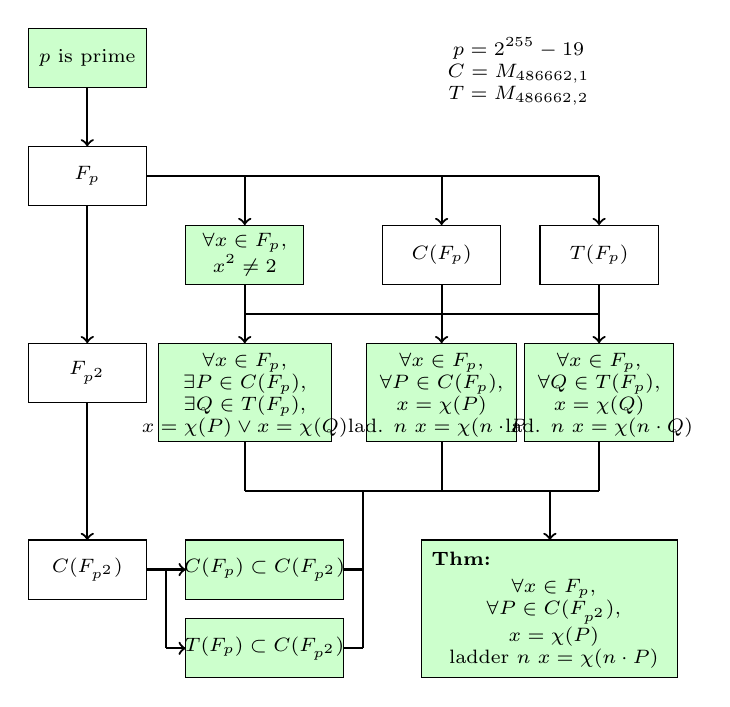
\begin{tikzpicture}[textstyle/.style={black, anchor= south west, align=center, minimum height=0.45cm, text centered, font=\scriptsize}]

  \draw (6.75,1.5) node[textstyle, anchor=north east] {$p = \p$\\$C = M_{486662,1}$\\$T = M_{486662,2}$\\};

  \begin{scope}[yshift=1.5 cm,xshift=-0.5 cm]
   \draw [fill=green!20] (0,0) -- (1.5,0) -- (1.5,-0.75) -- (0, -0.75) -- cycle;
   \draw (0.75,-0.375) node[textstyle, anchor=center] {$p$ is prime};
  \end{scope}

  \begin{scope}[yshift=0 cm,xshift=-0.5 cm]
   \draw[fill=white] (0,0) -- (1.5,0) -- (1.5,-0.75) -- (0, -0.75) -- cycle;
   \draw (0.75,-0.375) node[textstyle, anchor=center] {$\F{p}$};
  \end{scope}

  \begin{scope}[yshift=-1 cm,xshift=1.5 cm]
   \draw[fill=green!20] (0,0) -- (1.5,0) -- (1.5,-0.75) -- (0, -0.75) -- cycle;
   \draw (0.75,-0.375) node[textstyle, anchor=center] {$\forall x \in \F{p},$\\$x^2 \neq 2$};
  \end{scope}

  \begin{scope}[yshift=-1 cm,xshift=4 cm]
   \draw[fill=white] (0,0) -- (1.5,0) -- (1.5,-0.75) -- (0, -0.75) -- cycle;
   \draw (0.75,-0.375) node[textstyle, anchor=center] {$C(\F{p})$};
  \end{scope}

  \begin{scope}[yshift=-1 cm,xshift=6 cm]
   \draw[fill=white] (0,0) -- (1.5,0) -- (1.5,-0.75) -- (0, -0.75) -- cycle;
   \draw (0.75,-0.375) node[textstyle, anchor=center] {$T(\F{p})$};
  \end{scope}

  \path [thick, double, ->] (0.25,0.75) edge  [out=-90, in=90] (0.25,0);
  \path [thick, double]     (1,-0.375) edge  [out=0, in=180] (6.75,-0.375);
  \path [thick, double, ->] (2.25,-0.375) edge  [out=-90, in=90] (2.25,-1);
  \path [thick, double, ->] (4.75,-0.375) edge  [out=-90, in=90] (4.75,-1);
  \path [thick, double, ->] (6.75,-0.375) edge  [out=-90, in=90] (6.75,-1);


  \begin{scope}[yshift=-2.5 cm,xshift=1.5 cm]
   \draw[fill=green!20] (-0.35,0) -- (1.85,0) -- (1.85,-1.25) -- (-0.35, -1.25) -- cycle;
   \draw (0.75,0) node[textstyle, anchor=north] {$\forall x \in \F{p},$\\$\exists P \in C(\F{p}),$\\$\exists Q \in T(\F{p})$,\\$x = \chi(P)\vee x = \chi(Q)$};
  \end{scope}

  \begin{scope}[yshift=-2.5 cm,xshift=4 cm]
   \draw[fill=green!20] (-0.20,0) -- (1.70,0) -- (1.70,-1.25) -- (-0.20, -1.25) -- cycle;
   \draw (0.75,0) node[textstyle, anchor=north] {$\forall x \in \F{p},$\\$\forall P \in C(\F{p}),$\\$x = \chi(P)\implies$\\lad. $n$ $x = \chi(n \cdot P)$};
  \end{scope}

  \begin{scope}[yshift=-2.5 cm,xshift=6 cm]
   \draw[fill=green!20] (-0.20,0) -- (1.70,0) -- (1.70,-1.25) -- (-0.20, -1.25) -- cycle;
   \draw (0.75,0) node[textstyle, anchor=north] {$\forall x \in \F{p},$\\$\forall Q \in T(\F{p}),$\\$x = \chi(Q)\implies$\\lad. $n$ $x = \chi(n \cdot Q)$};
  \end{scope}

  \path [thick, double]     (2.25,-2.125) edge  [out=0, in=180] (6.75,-2.125);
  \path [thick, double, ->] (2.25,-1.75) edge  [out=-90, in=90] (2.25,-2.5);
  \path [thick, double, ->] (4.75,-1.75) edge  [out=-90, in=90] (4.75,-2.5);
  \path [thick, double, ->] (6.75,-1.75) edge  [out=-90, in=90] (6.75,-2.5);

% F(p^2)

  \path [thick, double, ->] (0.25,-0.75) edge  [out=-90, in=90] (0.25,-2.5);

  \begin{scope}[yshift=-2.5 cm,xshift=-0.5 cm]
   \draw[fill=white] (0,0) -- (1.5,0) -- (1.5,-0.75) -- (0, -0.75) -- cycle;
   \draw (0.75,-0.375) node[textstyle, anchor=center] {$\F{p^2}$};
  \end{scope}

  \path [thick, double, ->] (0.25,-3.25) edge  [out=-90, in=90] (0.25,-5);

  % C(F(p^2))

  \begin{scope}[yshift=-5 cm,xshift=-0.5 cm]
   \draw[fill=white] (0,0) -- (1.5,0) -- (1.5,-0.75) -- (0, -0.75) -- cycle;
   \draw (0.75,-0.375) node[textstyle, anchor=center] {$C(\F{p^2})$};
  \end{scope}

  \begin{scope}[yshift=-5 cm,xshift=1.5 cm]
   \draw[fill=green!20] (0,0) -- (2,0) -- (2,-0.75) -- (0, -0.75) -- cycle;
   \draw (1,-0.375) node[textstyle, anchor=center] {$C(\F{p}) \subset C(\F{p^2})$};
  \end{scope}

  \begin{scope}[yshift=-6 cm,xshift=1.5 cm]
   \draw[fill=green!20] (0,0) -- (2,0) -- (2,-0.75) -- (0, -0.75) -- cycle;
   \draw (1,-0.375) node[textstyle, anchor=center] {$T(\F{p}) \subset C(\F{p^2})$};
  \end{scope}

  \path [thick, double, ->] (1,-5.375) edge [out=0, in=-180] (1.5,-5.375);
  \path [thick, double] (1.25,-5.375) edge [out=-90, in=90] (1.25,-6.375);
  \path [thick, double, ->] (1.25,-6.375) edge [out=0, in=-180] (1.5,-6.375);

  \begin{scope}[yshift=-5 cm,xshift=4.5 cm]
    \draw [fill=green!20] (0,0) -- (3.25,0) -- (3.25,-1.75) -- (0, -1.75) -- cycle;
    \draw (0,0) node[textstyle, anchor=north west] {\textbf{Thm:}};
    \draw (1.675,-0.375) node[textstyle, anchor=north] {$\forall x \in \F{p},$\\$\forall P \in C(\F{p^2}),$\\$x = \chi(P)\implies$\\ladder $n$ $x = \chi(n \cdot P)$};
  \end{scope}

  \path [thick, double]     (2.25,-4.375) edge  [out=0, in=180] (6.75,-4.375);
  \path [thick, double]     (2.25,-3.75) edge  [out=-90, in=90] (2.25,-4.375);
  \path [thick, double]     (4.75,-3.75) edge  [out=-90, in=90] (4.75,-4.375);
  \path [thick, double]     (6.75,-3.75) edge  [out=-90, in=90] (6.75,-4.375);

  \path [thick, double]     (3.5,-5.375) edge  [out=0, in=180] (3.75,-5.375);
  \path [thick, double]     (3.5,-6.375) edge  [out=0, in=180] (3.75,-6.375);
  \path [thick, double]     (3.75,-6.375) edge  [out=90, in=-90] (3.75,-4.375);

  \path [thick, double, ->] (6.125,-4.375) edge [out=-90, in=90] (6.125,-5);

\end{tikzpicture}

  % \vspace{-0.5cm}
  \caption{Proof dependencies for the correctness of X25519.}
  \label{tikz:ProofHighLevel2}
\end{figure}

A brief overview of the complete proof is described below.
We first pose $a = 486662$, $b = 1$, $b' = 2$, $p = 2^{255}-19$, with the equations $C = M_{a,b}$, and $T = M_{a,b'}$.
We prove the primality of $p$ and define the field $\F{p}$.
Subsequently, we show that neither $2$ nor $a^2 - 2$ are square in $\F{p}$.
We consider $\F{p^2}$ and define $C(\F{p})$, $T(\F{p})$, and $C(\F{p^2})$.
We prove that for all $x \in \F{p}$ there exists a point of \xcoord $x$ either on $C(\F{p})$ or on the quadratic twist $T(\F{p})$.
We prove that all points in $M(\F{p})$ and $T(\F{p})$ can be projected in $M(\F{p^2})$ and derive that computations done in $M(\F{p})$ and $T(\F{p})$ yield to the same results if projected to $M(\F{p^2})$.
Using \tref{thm:montgomery-ladder-correct} we prove that the ladder is correct for $M(\F{p})$ and $T(\F{p})$; with the previous results, this results in the correctness of the ladder for $M(\F{p^2})$, in other words the correctness of X25519.

Now that we have an red line for the proof, we turn our attention to the details.
Indeed \tref{thm:montgomery-ladder-correct} cannot be applied directly to prove that X25519 is
doing the computations over $M(\F{p^2})$. This would infer that $\K = \F{p^2}$ and we would need to satisfy
hypothesis~\ref{hyp:a_minus_4_not_square}:%
% $a^2-4$ is not a square in \K:
$$\forall x \in \K,\ x^2 \neq a^2-4.$$
which is not possible as there always exists $x \in \F{p^2}$ such that $x^2 = a^2-4$.
Consequently, we first study Curve25519 and one of its quadratic twists Twist25519,
both defined over \F{p}.

\subsubsection{Curves and twists}
\label{subsec:Zmodp}

We define $\F{p}$ as the numbers between $0$ and $p = \p$.
We create a \coqe{Zmodp} module to encapsulate those definitions.
\begin{lstlisting}[language=Coq]
Module Zmodp.
Definition betweenb x y z := (x <=? z) && (z <? y).
Definition p := locked (2^255 - 19).
Fact Hp_gt0 : p > 0.
Inductive type := Zmodp x of betweenb 0 p x.
\end{lstlisting}

We define the basic operations ($+, -, \times$) with their respective neutral
elements ($0, 1$) and prove \lref{lemma:Zmodp_field}.
\begin{lemma}
  \label{lemma:Zmodp_field}
  $\F{p}$ is a field.
\end{lemma}
For $a = 486662$, by using the Legendre symbol we prove that
$a^2 - 4$ and $2$ are not squares in $\F{p}$.
% \begin{lstlisting}[language=Coq,belowskip=-0.25 \baselineskip]
% Fact a_not_square : forall x: Zmodp.type,
%   x^+2 != (Zmodp.pi 486662)^+2 - 4%:R.
% \end{lstlisting}
% \begin{lstlisting}[language=Coq,label=two_not_square,belowskip=-0.1 \baselineskip]
% Fact two_not_square : forall x: Zmodp.type,
%   x^+2 != 2%:R.
% \end{lstlisting}
This allows us to study $M_{486662,1}(\F{p})$ and $M_{486662,2}(\F{p})$, one of its quadratic twists.
% \begin{dfn}Let the following instantiations of \aref{alg:montgomery-double-add}:\\
\begin{dfn}
  %Let the following instantiations of \aref{alg:montgomery-ladder}:\\
  We instantiate \coqe{opt_montgomery} in two specific ways:
  \begin{itemize}
    \item[--] $Curve25519\_Fp(n,x)$ for $M_{486662,1}(\F{p})$.
    \item[--] $Twist25519\_Fp(n,x)$ for $M_{486662,2}(\F{p})$.
  \end{itemize}
\end{dfn}

With \tref{thm:montgomery-ladder-correct} we derive the following two lemmas:
\begin{lemma}
  For all $x \in \F{p},\ n \in \N,\ P \in \F{p} \times \F{p}$,\\
  such that $P \in M_{486662,1}(\F{p})$ and $\chi_0(P) = x$.
  $$Curve25519\_Fp(n,x) = \chi_0(n \cdot P)$$
\end{lemma}
\begin{lemma}
  For all $x \in \F{p},\ n \in \N,\ P \in \F{p} \times \F{p}$\\
  such that $P \in M_{486662,2}(\F{p})$ and $\chi_0(P) = x$.
  $$Twist25519\_Fp(n,x) = \chi_0(n \cdot P)$$
\end{lemma}
As the Montgomery ladder does not depend on $b$, it is trivial to
see that the computations done for points in $M_{486662,1}(\F{p})$ and in
$M_{486662,2}(\F{p})$ are the same.
% \begin{lstlisting}[language=Coq]
% Theorem curve_twist_eq: forall n x,
%   curve25519_Fp_ladder n x = twist25519_Fp_ladder n x.
% \end{lstlisting}

Because $2$ is not a square in $\F{p}$, it allows us split $\F{p}$ into two sets.
\begin{lemma}
  \label{lemma:square-or-2square}
  For all $x$ in $\F{p}$, there exists $y$ in $\F{p}$ such that
  $$y^2 = x\ \ \ \lor\ \ 2y^2 = x$$
\end{lemma}
For all $x \in \F{p}$, we can compute $x^3 + ax^2 + x$. Using \lref{lemma:square-or-2square}
we can find a $y$ such that $(x,y)$ is either on the curve or on the quadratic twist:
\begin{lemma}
  \label{lemma:curve-or-twist}
  For all $x \in \F{p}$, there exists a point $P$ in $M_{486662,1}(\F{p})$ or
  in $M_{486662,2}(\F{p})$ such that the \xcoord of $P$ is $x$.
\end{lemma}
\begin{lstlisting}[language=Coq,belowskip=-0.5 \baselineskip]
Theorem x_is_on_curve_or_twist:
  forall x : Zmodp.type,
  (exists (p : mc curve25519_mcuType), p#x0 = x) \/
  (exists (p' : mc twist25519_mcuType), p'#x0 = x).
\end{lstlisting}

\subsubsection{Curve25519 over \F{p^2}}
\label{subsec:curvep2}

The quadratic extension $\F{p^2}$ is defined as $\F{p}[\sqrt{2}]$ by~\cite{Ber06}.
The theory of finite fields already has been formalized in the Mathematical Components
library,
%ref?
but this formalization is rather abstract, and we need concrete representations of field
elements here.
For this reason we decided to formalize a definition of $\F{p^2}$ ourselves.

We can represent $\F{p^2}$ as the set $\F{p} \times \F{p}$,
% in other words,
representing polynomials with coefficients in $\F{p}$ modulo $X^2 - 2$. In a similar way
as for $\F{p}$ we use a module in Coq.
\begin{lstlisting}[language=Coq,belowskip=-0.25 \baselineskip]
Module Zmodp2.
Inductive type :=
  Zmodp2 (x: Zmodp.type) (y:Zmodp.type).

Definition pi (x: Zmodp.type * Zmodp.type) : type :=
  Zmodp2 x.1 x.2.
Definition mul (x y: type) : type :=
  pi ((x.1 * y.1) + (2%:R * (x.2 * y.2)),
      (x.1 * y.2) + (x.2 * y.1)).
\end{lstlisting}
% Definition zero : type :=
%   pi ( 0%:R, 0%:R ).
% Definition one : type :=
%   pi ( 1, 0%:R ).
% Definition opp (x: type) : type :=
%   pi (- x.1 , - x.2).
% Definition add (x y: type) : type :=
%   pi (x.1 + y.1, x.2 + y.2).
% Definition sub (x y: type) : type :=
%   pi (x.1 - y.1, x.2 - y.2).

We define the basic operations ($+, -, \times$) with their respective neutral
elements $0$ and $1$. Additionally we verify that for each element of in
$\F{p^2}\backslash\{0\}$, there exists a multiplicative inverse.
\begin{lemma}
  \label{lemma:Zmodp2_inv}
  For all $x \in \F{p^2}\backslash\{0\}$ and $a,b \in \F{p}$ such that $x = (a,b)$,
  $$x^{-1} = \Big(\frac{a}{a^2-2b^2}\ , \frac{-b}{a^2-2b^2}\Big)$$
\end{lemma}
As in $\F{p}$, we define $0^{-1} = 0$ and prove \lref{lemma:Zmodp2_field}.
\begin{lemma}
  \label{lemma:Zmodp2_field}
  $\F{p^2}$ is a commutative field.
\end{lemma}

%% TOO LONG
%% If need remove this paragraph
We then specialize the basic operations in order to speed up the verification
of formulas by using rewrite rules:
\begin{equation*}
  \begin{split}
    (a,0) + (b,0) &= (a+b, 0)\\[-0.5ex]
    (a, 0)^{-1} &= (a^{-1}, 0)
  \end{split}
  \qquad
  \begin{split}
    (a,0) \cdot   (b,0) &= (a \cdot b, 0)\\[-0.5ex]
    (0,a)^{-1} &= (0,(2\cdot a)^{-1})
  \end{split}
\end{equation*}

The injection $a \mapsto (a,0)$ from $\F{p}$ to $\F{p^2}$ preserves
$0, 1, +, -, \times$. Thus $(a,0)$ can be abbreviated as $a$ without confusion.

We define $M_{486662,1}(\F{p^2})$. With the rewrite rule above, it is straightforward
to prove that any point on the curve $M_{486662,1}(\F{p})$ is also on the curve
$M_{486662,1}(\F{p^2})$. Similarly, any point on the quadratic twist
$M_{486662,2}(\F{p})$ also corresponds to a point on the curve $M_{486662,1}(\F{p^2})$.
As direct consequence, using \lref{lemma:curve-or-twist}, we prove that for all
$x \in \F{p}$, there exists a point $P \in \F{p^2}\times\F{p^2}$ on
$M_{486662,1}(\F{p^2})$ such that $\chi_0(P) = (x,0) = x$.

\begin{lstlisting}[language=Coq,belowskip=-0.25 \baselineskip]
Lemma x_is_on_curve_or_twist_implies_x_in_Fp2:
  forall (x:Zmodp.type),
    exists (p: mc curve25519_Fp2_mcuType),
      p#x0 = Zmodp2.Zmodp2 x 0.
\end{lstlisting}

We now study the case of the scalar multiplication and show similar proofs.
\begin{dfn}
  Define the functions $\varphi_c$, $\varphi_t$ and $\psi$
  \begin{itemize}
    \item[--] $\varphi_c: M_{486662,1}(\F{p}) \mapsto M_{486662,1}(\F{p^2})$\\
          such that $\varphi((x,y)) = ((x,0), (y,0))$.
    \item[--] $\varphi_t: M_{486662,2}(\F{p}) \mapsto M_{486662,1}(\F{p^2})$\\
          such that $\varphi((x,y)) = ((x,0), (0,y))$.
    \item[--] $\psi: \F{p^2} \mapsto \F{p}$ such that $\psi(x,y) = x$.
  \end{itemize}
\end{dfn}

\begin{lemma}
  \label{lemma:proj}
  For all $n \in \N$, for all point $P\in\F{p}\times\F{p}$ on the curve
  $M_{486662,1}(\F{p})$ (respectively on the quadratic twist $M_{486662,2}(\F{p})$), we have
  \vspace{-0.3em}
  \begin{align*}
    P & \in M_{486662,1}(\F{p}) & \implies \varphi_c(n \cdot P) & = n \cdot \varphi_c(P), &  & \text{and} \\[-0.5ex]
    P & \in M_{486662,2}(\F{p}) & \implies \varphi_t(n \cdot P) & = n \cdot \varphi_t(P).
  \end{align*}
\end{lemma}
Notice that
\vspace{-0.5em}
\begin{align*}
  \forall P \in M_{486662,1}(\F{p}), &  & \psi(\chi_0(\varphi_c(P))) & = \chi_0(P), &  & \text{and} \\[-0.5ex]
  \forall P \in M_{486662,2}(\F{p}), &  & \psi(\chi_0(\varphi_t(P))) & = \chi_0(P).
\end{align*}

In summary, for all $n \in \N$, $n < 2^{255}$, for any point $P\in\F{p}\times\F{p}$
in $M_{486662,1}(\F{p})$ or $M_{486662,2}(\F{p})$, $Curve25519\_Fp$
computes $\chi_0(n \cdot P)$.
We have proved that for all $P \in \F{p^2}\times\F{p^2}$ such that $\chi_0(P) \in \F{p}$,
there exists a corresponding point on the curve or the twist over $\F{p}$.
Moreover, we have proved that for any point on the curve or the twist, we can compute the
scalar multiplication by $n$ and obtain the same result as if we did the
computation in $\F{p^2}$.
% As a result we have proved theorem 2.1 of \cite{Ber06}:
% No: missing uniqueness !
\begin{theorem}
  \label{thm:general-scalarmult}
  For all $n \in \N$, such that $n < 2^{255}$,
  for all $x \in \F{p}$ and $P \in M_{486662,1}(\F{p^2})$ such that $\chi_0(P) = x$,
  $Curve25519\_Fp(n,x)$ computes $\chi_0(n \cdot P)$.
\end{theorem}
% which is formalized in Coq as:
% \begin{lstlisting}[language=Coq,belowskip=-0.1 \baselineskip]
% Theorem curve25519_Fp2_ladder_ok:
%   forall (n : nat) (x:Zmodp.type),
%   (n < 2^255)%nat ->
%   forall (p  : mc curve25519_Fp2_mcuType),
%   p #x0 = Zmodp2.Zmodp2 x 0 ->
%   curve25519_Fp_ladder n x = (p *+ n)#x0 /p.
% \end{lstlisting}

We then prove the equivalence of operations between $\Ffield$ and $\Zfield$,
in other words between \coqe{Zmodp} and \coqe{:GF}.
This allows us to show that given a clamped value $n$ and normalized \xcoord of $P$,
\coqe{RFC} gives the same results as $Curve25519\_Fp$.

All put together, this finishes the proof of the mathematical correctness of X25519: the fact that the code in X25519, both in the RFC~7748 and
in TweetNaCl versions, correctly computes multiplication in the elliptic curve.

\section{Conclusion}
\label{sec:Conclusion}

Any formal system relies on a trusted base. In this section we describe our
chain of trust.

\subheading{Trusted Code Base of the proof.}
Our proof relies on a trusted base, i.e. a foundation of definitions that must be
correct. One should not be able to prove a false statement in that system, \eg by
proving an inconsistency.

In our case we rely on:
\begin{itemize}
      \item \textbf{Calculus of Inductive Constructions}. The intuitionistic logic
            used by Coq must be consistent in order to trust the proofs. As an axiom,
            we assume that the functional extensionality is also consistent with that logic.
            $$\forall x, f(x) = g(x) \implies f = g$$
%             \begin{lstlisting}[language=Coq,belowskip=-0.25 \baselineskip]
% Lemma f_ext: forall (A B:Type),
%   forall (f g: A -> B),
%   (forall x, f(x) = g(x)) -> f = g.
% \end{lstlisting}

      \item \textbf{Verifiable Software Toolchain}. This framework developed at
            Princeton allows a user to prove that a Clight code matches pure Coq
            specification.

      \item \textbf{CompCert}. When compiling with CompCert we only need to trust
            CompCert's {assembly} semantics, as the compilation chain has been formally proven correct.
            However, when compiling with other C compilers like Clang or GCC, the
            whole code base of these compilers becomes part of the TCB.

      \item \textbf{\texttt{clightgen}}. The tool translating from {C} to
                  {Clight}, the first step of the CompCert compilation.
            This compilation step is not covered by the proofs of CompCert
            and VST requires Clight input. For example, VST does not support the direct verification of
            \texttt{o[i] = a[i] + b[i]}, which \texttt{clightgen} translates to
            \begin{lstlisting}[language=Ctweetnacl,stepnumber=0,belowskip=-0.5 \baselineskip]
aux1 = a[i]; aux2 = b[i];
o[i] = aux1 + aux2;
\end{lstlisting}
            The \texttt{-normalize} flag is taking care of this
            rewriting and factors out assignments from inside subexpressions.
            % The trust of the proof relies on a correct translation from the
            % initial version of \emph{TweetNaCl} to \emph{TweetNaClVerifiableC}.
            % The changes required for C code to make it verifiable are now minimal.

      \item Finally, we must trust the \textbf{Coq kernel} and its
            associated libraries; the \textbf{Ocaml compiler} on which we compiled Coq;
            the \textbf{Ocaml Runtime} and the \textbf{CPU}. Those are common to all proofs
            done with this architecture \cite{2015-Appel,coq-faq}.
\end{itemize}

\subheading{Corrections in TweetNaCl.}
As a result of this verification, we removed superfluous code.
Indeed indexes 17 to 79 of the \TNaCle{i64 x[80]} intermediate variable of
\TNaCle{crypto_scalarmult} were adding unnecessary complexity to the code,
we removed them.

Wu and Donenfeld brought to our attention that the original
\TNaCle{car25519} function carried a risk of undefined behavior if \texttt{c}
is a negative number.
\begin{lstlisting}[language=Ctweetnacl,stepnumber=0]
c=o[i]>>16;
o[i]-=c<<16; // c < 0 = UB !
\end{lstlisting}
We replaced this statement with a logical \texttt{and}, proved correctness,
and thus solved this problem.
\begin{lstlisting}[language=Ctweetnacl,stepnumber=0]
o[i]&=0xffff;
\end{lstlisting}

Aside from this modifications, all subsequent alterations to the TweetNaCl code%
---such as the type change of loop indexes (\TNaCle{int} instead of \TNaCle{i64})---%
were required for VST to step through the code properly. We believe that those
adjustments do not impact the trust of our proof.

We contacted the authors of TweetNaCl and expect that the changes described
above will soon be integrated in a new version of the library.


% Do we want to say that ?

% \subheading{Verification Effort.}
% In addition to the time required to get familiar with
% research software, we faced a few bugs which we reported
% to the developers of VST to get them fixed.
% It is very hard to work with a tool without being involved
% in the development loop. Additionally newer versions often
% broke some of our proofs and it was often needed to adapt
% to the changes.
% As a result we do not believe the metric person-month to be
% a good representation of the verification effort.

\subheading{Lessons learned.}
Most efforts in the area of high-assurance crypto are carried out
by teams who at the same time work on tools and proofs and often
even co-develop the implementations with the proofs.
In this effort we set out to verify pre-existing software,
written in a not particularly verification-friendly language
using a set of tools (VST and Coq) whose development we are not
actively involved in.

TweeNaCl comes with a claim of verifiability, but it became clear
rather quickly that this claim is only based on the overall simplicity
of the library and not supported by code written carefully such that it can
efficiently be verified with existing tools. The difference between
our verified version of TweetNaCl and the original TweetNaCl in
Appendix~\ref{verified-C-and-diff} gives an idea of some minimal
changes we had to apply to work with VST; many more small changes
would have made the proof much easier and more elegant. As one
example, in \TNaCle{pack25519} the substraction of $p$ and the carry
propagation are done in a single \TNaCle{for} loop;
had they been splitted into two loops, the final result would have been the same with a
verification effort significantly lessen.

There were many positive lessons to be learned from this verification effort;
most importantly that it is possible to prove ``legacy'' cryptographic
software written in C correct without having to co-develop proofs
and tools. However, we also learned that it is still necessary to
understand to some extent how these tools (in particular VST)
work under the hood.
VST is a collection of lemmas and proof tactics; the idea is
to expose the user only to the tactics and hide the details of
the underlying lemmas.
At least in the VST versions we worked with,
this approach did not quite work and at various stages in
the proofs we had to look into the underlying lemmas.
This was due to the provided tactics not terminating,
for example in the last few steps \coqe{pack25519}'s VST proof.
Some struggle with VST also taught us another very pleasant lesson,
namely that the VST development team is very responsive and helpful.
Various of our issues were sorted out with their help and we hope
that some of the experience we brought in also helped improve VST.

\subheading{Extending our work.}
The high-level definition (\sref{sec:maths}) can easily be ported to any
other Montgomery curves and with it the proof of the ladder's correctness
assuming the same formulas are used.
In addition to the curve equation, the field \F{p} would need to be redefined
as $p=2^{255}-19$ is hard-coded in order to speed up some proofs.

With respect to the C code verification (\sref{sec:C-Coq}), the extension of
the verification effort to Ed25519 would make directly use of the low-level
arithmetic. The ladder steps formula being different this would require a high
level verification similar to \tref{thm:montgomery-ladder-correct};
also, a full correctness verification of Ed25519 signatures would require
verifying correctness of SHA-512.

The verification of \eg X448~\cite{cryptoeprint:2015:625,rfc7748} in C would
require the adaptation of most of the low-level arithmetic (mainly the
multiplication, carry propagation and reduction).
Once the correctness and bounds of the basic operations are established,
reproving the full ladder would make use of our generic definition.

\subheading{A complete proof.}
We provide a mechanized formal proof of the correctness of the X25519
implementation in TweetNaCl from C up the mathematical definitions with a single tool.
We first formalized X25519 from RFC~7748~\cite{rfc7748} in Coq.
We then proved that TweetNaCl's implementation of X25519 matches our formalization.
In a second step we extended the Coq library for elliptic curves \cite{BartziaS14}
by Bartzia and Strub to support Montgomery curves.
Using this extension we proved that the X25519 from the RFC matches the
mathematical definitions as given in~\cite[Sec.~2]{Ber06}.
Therefore in addition to proving the mathematical correctness of TweetNaCl,
we also increases the trust of other works such as
\cite{zinzindohoue2017hacl,Erbsen2016SystematicSO} which rely on RFC~7748.
\vspace{-0.3cm}

\bibliographystyle{IEEEtran}
\bibliography{collection}

\begin{appendices}
  \section{The complete X25519 code from TweetNaCl}
\label{verified-C-and-diff}

\subheading{Verified C Code} We provide below the code we verified.

\lstinputlisting[linerange={2-5,8-9,266-317,333-380,393-438},language=Ctweetnacl]{../proofs/vst/c/tweetnaclVerifiableC.c}
~

\subheading{Diff from TweetNaCl} We provide below the diff between the original code of TweetNaCl and the code we verified.

\lstinputlisting[language=diff]{tweetnacl.diff}

As follow, we provide the explanations of the above changes to TweetNaCl's code.

\begin{itemize}
  \item lines 7-8: We tell VST that \TNaCle{long long} are
  aligned on 8 bytes.

  \item lines 16-23: We remove the the undefined behavior as explained in \sref{sec:Conclusion}.

  \item lines 29-31; lines 60-62: VST does not support \TNaCle{for} loops over \TNaCle{i64}, we convert it into an \TNaCle{int}.

  \item lines 39 \& 41: We initialize \TNaCle{m} with \TNaCle{0}.
  This change allows us to prove the functional correctness of \TNaCle{pack25519} without having to deal with an array containing
  a mix of uninitialized and initialized values.
  A hand iteration over the loop trivially shows that no uninitialized values are used.

  \item lines 40 \& 42; lines 70 \& 71: We replace the \TNaCle{FOR} loop by \TNaCle{set25519}. The code is the same once the function is inlined. This small change is purely cosmetic but stays in the spirit of tweetnacl: keeping a small code size while being auditable.

  \item lines 50-52: VST does not allow computation in the argument before a function call. Additionally \texttt{clightgen} does not extract the computation either. We add this small step to allow VST to carry through the proof.

  % \item lines 60-62: VST does not support \TNaCle{for} loops over \TNaCle{i64}, we convert it into an \TNaCle{int}.

  % \item lines 70-71: We replace \TNaCle{FOR(a,16) c[a]=i[a];} by \TNaCle{set25519(c,i);}. The semantic of operation done is the same once \TNaCle{set25519} is inlined. This small change is purely cosmetic but stays in the spirit of tweetnacl: keeping a small code size while being auditable.

  \item lines 79-82: VST does not support \TNaCle{for} loops over \TNaCle{i64}, we convert it into an \TNaCle{int}.\\
  In the function calls of \TNaCle{sel25519}, the specifications requires the use of \TNaCle{int}, the value of \TNaCle{r} being either \TNaCle{0} or \TNaCle{1}, we consider this change safe.

  \item Lines 90-101: The \TNaCle{for} loop does not add any benefits to the code. By removing it we simplify the source and the verification steps as we do not need to deal with pointer arithmetic. Thus, \TNaCle{x} is limited to only 16 \TNaCle{i64}, \ie \TNaCle{gf}.

\end{itemize}

  \subsection{Coq definitions}
\label{appendix:coq}

\subsubsection{Montgomery Ladder}
\label{subsubsec:coq-ladder}

Generic definition of the ladder:

\begin{lstlisting}[language=Coq]
(* Typeclass to encapsulate the operations *)
Class Ops (T T': Type) (Mod: T -> T):=
{
  +   : T -> T -> T;           (* Add           *)
  *   : T -> T -> T;           (* Mult          *)
  -   : T -> T -> T;           (* Sub           *)
  x^2  : T -> T;                (* Square        *)
  C_0 : T;                     (* Constant 0    *)
  C_1 : T;                     (* Constant 1    *)
  C_121665: T;                 (* const (a-2)/4 *)
  Sel25519: Z -> T -> T -> T; (* CSWAP         *)
  Getbit: Z -> T' -> Z;       (* ith bit       *)
}.

Fixpoint montgomery_rec (m : nat) (z : T')
(a: T) (b: T) (c: T) (d: T) (e: T) (f: T) (x: T) :
(* a: x2              *)
(* b: x3              *)
(* c: z2              *)
(* d: z3              *)
(* e: temporary  var  *)
(* f: temporary  var  *)
(* x: x1              *)
(T * T * T * T * T * T) :=
match m with
| 0%nat => (a,b,c,d,e,f)
| S n =>
  let r := Getbit (Z.of_nat n) z in
    (* k_t = (k >> t) & 1                       *)
    (* swap <- k_t                              *)
  let (a, b) := (Sel25519 r a b, Sel25519 r b a) in
    (* (x_2, x_3) = cswap(swap, x_2, x_3)            *)
  let (c, d) := (Sel25519 r c d, Sel25519 r d c) in
    (* (z_2, z_3) = cswap(swap, z_2, z_3)            *)
  let e := a + c in  (* A = x_2 + z_2              *)
  let a := a - c in  (* B = x_2 - z_2              *)
  let c := b + d in  (* C = x_3 + z_3              *)
  let b := b - d in  (* D = x_3 - z_3              *)
  let d := e ^2 in    (* AA = A^2                  *)
  let f := a ^2 in    (* BB = B^2                  *)
  let a := c * a in  (* CB = C * B               *)
  let c := b * e in  (* DA = D * A               *)
  let e := a + c in  (* x_3 = (DA + CB)^2          *)
  let a := a - c in  (* z_3 = x_1 * (DA - CB)^2     *)
  let b := a ^2 in    (* z_3 = x_1 * (DA - CB)^2     *)
  let c := d - f in  (* E = AA - BB             *)
  let a := c * C_121665 in
                     (* z_2 = E * (AA + a24 * E) *)
  let a := a + d in  (* z_2 = E * (AA + a24 * E) *)
  let c := c * a in  (* z_2 = E * (AA + a24 * E) *)
  let a := d * f in  (* x_2 = AA * BB            *)
  let d := b * x in  (* z_3 = x_1 * (DA - CB)^2    *)
  let b := e ^2 in    (* x_3 = (DA + CB)^2         *)
  let (a, b) := (Sel25519 r a b, Sel25519 r b a) in
    (* (x_2, x_3) = cswap(swap, x_2, x_3)           *)
  let (c, d) := (Sel25519 r c d, Sel25519 r d c) in
    (* (z_2, z_3) = cswap(swap, z_2, z_3)           *)
  montgomery_rec n z a b c d e f x
end.

Definition get_a (t:(T * T * T * T * T * T)) : T :=
match t with
  (a,b,c,d,e,f) => a
end.
Definition get_c (t:(T * T * T * T * T * T)) : T :=
match t with
  (a,b,c,d,e,f) => c
end.
\end{lstlisting}

\subsubsection{Equivalence between For Loops}
\label{subsubsec:for}

\begin{lstlisting}[language=Coq]
Variable T: Type.
Variable g: nat -> T -> T.

Fixpoint rec_fn (n:nat) (s:T) :=
  match n with
  | 0 => s
  | S n => rec_fn n (g n s)
  end.

Fixpoint rec_fn_rev_acc (n:nat) (m:nat) (s:T) :=
  match n with
  | 0 => s
  | S n => g (m - n - 1) (rec_fn_rev_acc n m s)
  end.

Definition rec_fn_rev (n:nat) (s:T) :=
  rec_fn_rev_acc n n s.

Lemma Tail_Head_equiv :
  forall (n:nat) (s:T),
  rec_fn n s = rec_fn_rev n s.
\end{lstlisting}

  \section{Organization of the proof files}
\label{appendix:proof-folders}

\subheading{Requirements.}
Our proofs requires the use of \emph{Coq 8.8.2} for the proofs and
\emph{Opam 2.0} to manage the dependencies. We are aware that there exists more
recent versions of Coq; VST; CompCert etc. however to avoid dealing with backward
breaking compatibility we decided to freeze our dependencies.

\subheading{Associated files.}
The repository containing the proof is composed of two folders \textbf{\texttt{packages}}
and \textbf{\texttt{proofs}}.
It aims to be used at the same time as an \emph{opam} repository to manage
the dependencies of the proof and to provide the code.

The actual proofs can be found in the \textbf{\texttt{proofs}} folder in which
the reader will find the directories \textbf{\texttt{spec}} and \textbf{\texttt{vst}}.

\subheading{\texttt{packages/}}
This folder makes sure that we are using the correct version of
Verifiable Software Toolchain (version 2.0) and CompCert (version 3.2).
Additionally it pins the version of the elliptic curves library by Bartzia and Strub
and allows us to use the theorem of quadratic reciprocity.

\subheading{\texttt{proofs/spec/}}
In this folder the reader will find multiple levels of implementation of X25519.
\begin{itemize}
  \item \textbf{\texttt{Libs/}} contains basic libraries and tools to help use
        reason with lists and decidable procedures.
  \item \textbf{\texttt{ListsOp/}} defines operators on list such as
        \Coqe{ZofList} and related lemmas using \eg \VSTe{Forall}.
  \item \textbf{\texttt{Gen/}} defines a generic Montgomery ladder which can be
        instantiated with different operations. This ladder is the stub for the
        following implementations.
  \item \textbf{\texttt{High/}} contains the theory of Montgomery curves,
        twists, quadratic extensions and ladder.
        It also proves the correctness of the ladder over $\F{\p}$.
  \item \textbf{\texttt{Mid/}} provides a list-based implementation of the
        basic operations \TNaCle{A}, \TNaCle{Z}, \TNaCle{M} \ldots~and the ladder. It
        makes the link with the theory of Montgomery curves.
  \item \textbf{\texttt{Low/}} provides a second list-based implementation of
        the basic operations \TNaCle{A}, \TNaCle{Z}, \TNaCle{M} \ldots~and the ladder.
        Those functions are proven to provide the same results as the ones in
        \texttt{Mid/}, however their implementation are closer to \texttt{C} in order
        facilitate the proof of equivalence with TweetNaCl code.
  \item \textbf{\texttt{rfc/}} provides our rfc formalization.
        It uses integers for the basic operations \TNaCle{A}, \TNaCle{Z}, \TNaCle{M}
        \ldots and the ladder. It specifies the decoding/encoding of/to byte
        arrays (seen as list of integers) as in RFC~7748.
\end{itemize}

\subheading{\texttt{proofs/vst/}}
Here the reader will find four folders.
\begin{itemize}
  \item \textbf{\texttt{c}} contains the C Verifiable implementation of TweetNaCl.
        \texttt{clightgen} will generate the appropriate translation into Clight.
  \item \textbf{\texttt{init}} contains basic lemmas and memory manipulation
        shortcuts to handle the aliasing cases.
  \item \textbf{\texttt{spec}} defines as Hoare triple the specification of the
        functions used in \TNaCle{crypto_scalarmult}.
  \item \textbf{\texttt{proofs}} contains the proofs of the above Hoare triples
        and thus the proof that TweetNaCl code is sound and correct.
\end{itemize}

\end{appendices}

\end{document}
